\documentclass[a4paper,10pt]{article}
\usepackage{tikz}
\usepackage{verbatim}
\usepackage[margin=15mm]{geometry}
\usetikzlibrary{shapes,arrows,fit,calc,positioning,intersections,backgrounds}


\begin{document}

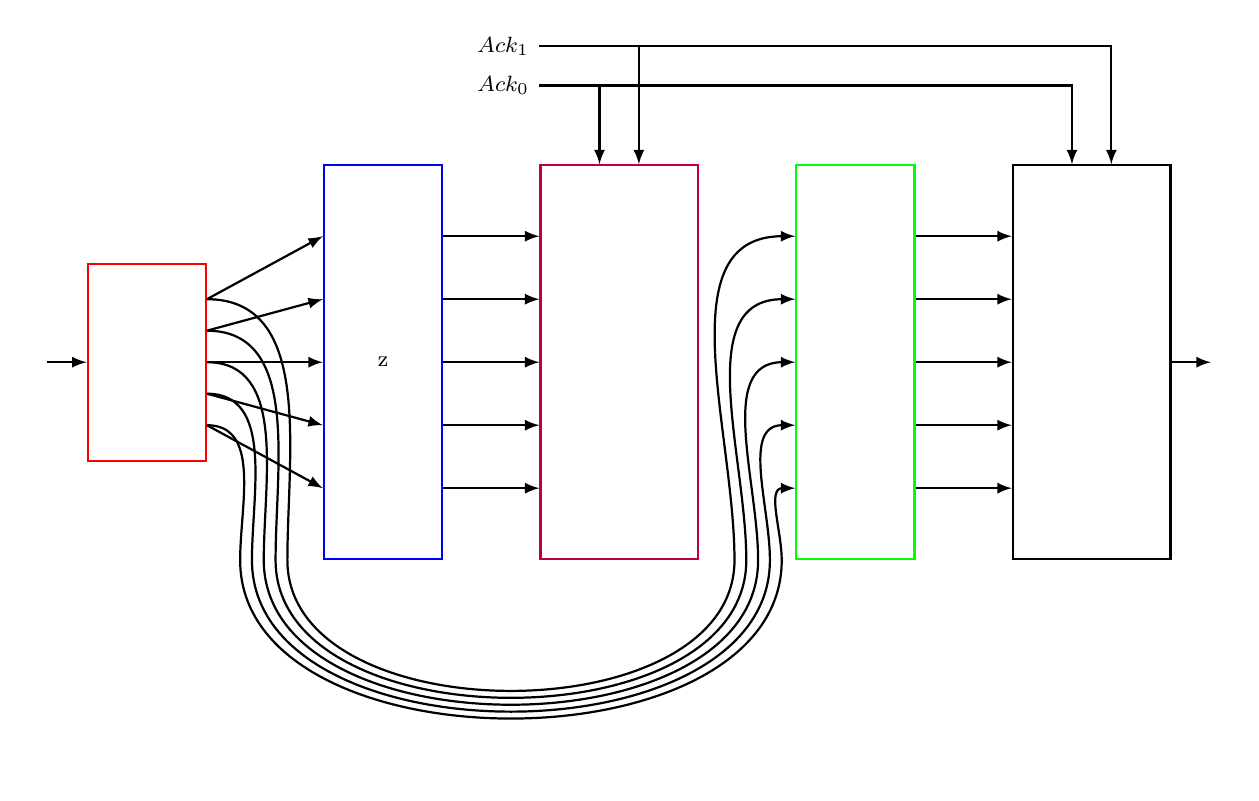
\begin{tikzpicture}[thick]
\tikzset{input/.style={}}
\tikzset{block/.style={rectangle,draw}}
\tikzstyle{pinstyle} = [pin edge={to-,thick,black}]

\node [input, name=input] {};
\node [block, right=0.5 cm of input,minimum width=1.5cm, minimum height=2.5cm,red] (a) {};
\node [block, right of=a,minimum width=1.5cm, minimum height=5cm,node distance=3cm,blue] (b) {};
\node [block, right of=b, minimum width=2cm, minimum height=5cm,node distance=3cm,purple] (c) {};
\node [block, right of=c,minimum width=1.5cm, minimum height=5cm,node distance=3cm,green] (d) {};
\node [block, right of=d, minimum width=2cm, minimum height=5cm,node distance=3cm] (e) {};
\node [right =0.5 cm of e] (output) {};

\begin{scope}[->,>=latex]

\draw[->] (input) -- (a);

\node at (b.center) {\footnotesize{z}};

\draw[->] ([yshift=1.5 cm]c.north west) node[left]{\footnotesize{$Ack_1$}} -| ([xshift=0.25 cm]e.north);
\draw[->] ([yshift=1.5 cm]c.north west) -| ([xshift=0.25 cm]c.north);
\draw[->] ([yshift=1 cm]c.north west) node[left]{\footnotesize{$Ack_0$}} -| ([xshift=-0.25 cm]e.north);
\draw[->] ([yshift=1 cm]c.north west) -| ([xshift=-0.25 cm]c.north);
\draw[->] (e) -- (output);

\foreach \i in {2,...,-2}{%
\draw[->] ([yshift=\i * 0.4 cm]a.east) -- ([yshift=\i * 0.8 cm]b.west) ;}

\foreach \i in {-2,...,2}{%
\draw[->] ([yshift=\i * 0.8 cm,]b.east) -- ([yshift=\i * 0.8 cm]c.west) ;}

\foreach \i in {-2,...,2}{%
\draw[->] ([yshift=\i * 0.4 cm]a.east) to [out=-0,in=90]  ([xshift={\i * 0.15 cm-0.75cm}]b.south west) to [out=-90,in=-90]  ([xshift={-\i * 0.15 cm+0.75cm}]c.south east)  to [out=90,in=-180]  ([yshift=\i * 0.8 cm]d.west) ;}

\foreach \i in {-2,...,2}{%
\draw[->] ([yshift=\i * 0.8 cm]d.east) -- ([yshift=\i * 0.8 cm]e.west) ;}

\end{scope}
\end{tikzpicture}



\begin{tikzpicture}
  \node[anchor=east] at (0,0) (text) {This is some text.};
  \node[anchor=west] at (3,1) (description) {Here is the description.};
  \draw (description) edge[out=180,in=0,->] (text);
\end{tikzpicture}

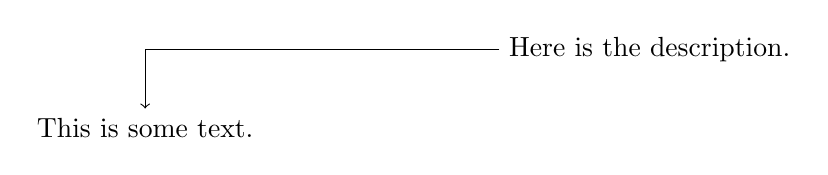
\begin{tikzpicture}
  \node[anchor=east] at (0,0) (text) {This is some text.};
  \node[anchor=west] at (3,1) (description) {Here is the description.};
  \draw[->] (description) -| (text);
\end{tikzpicture}


\begin{tikzpicture}
  \node[anchor=east] at (0,0) (text) {This is some text.};
  \node[anchor=west] at (3,1) (description) {Here is the description.};
  \draw[->] (description) .. controls ([xshift=-4cm] description) and ([xshift=4cm] text) .. (text);
\end{tikzpicture}


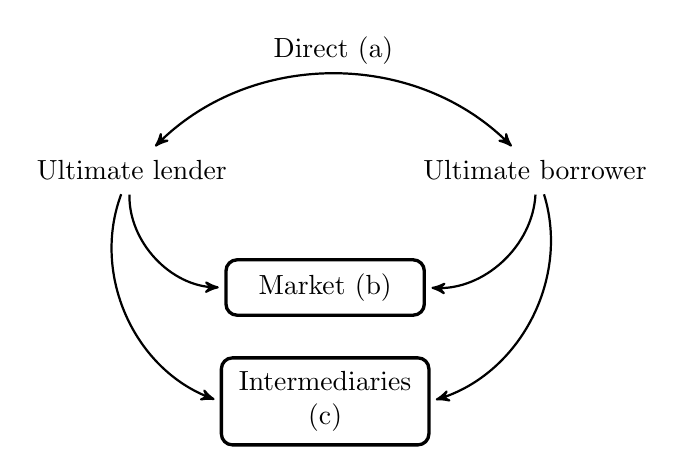
\begin{tikzpicture}[node distance=1cm, auto,]
\tikzset{
    %Define standard arrow tip
    >=stealth',
    %Define style for boxes
    punkt/.style={
           rectangle,
           rounded corners,
           draw=black, very thick,
           text width=6.5em,
           minimum height=2em,
           text centered},
    % Define arrow style
    pil/.style={
           ->,
           thick,
           shorten <=2pt,
           shorten >=2pt,}
}
 %nodes
 \node[punkt] (market) {Market (b)};
 \node[punkt, inner sep=5pt,below=0.5cm of market]
 (formidler) {Intermediaries (c)};
 % We make a dummy figure to make everything look nice.
 \node[above=of market] (dummy) {};
 \node[right=of dummy] (t) {Ultimate borrower}
   edge[pil,bend left=45] (market.east) % edges are used to connect two nodes
   edge[pil, bend left=45] (formidler.east); % .east since we want
                                             % consistent style
 \node[left=of dummy] (g) {Ultimate lender}
   edge[pil, bend right=45] (market.west)
   edge[pil, bend right=45] (formidler.west)
   edge[pil,<->, bend left=45] node[auto] {Direct (a)} (t);
\end{tikzpicture}


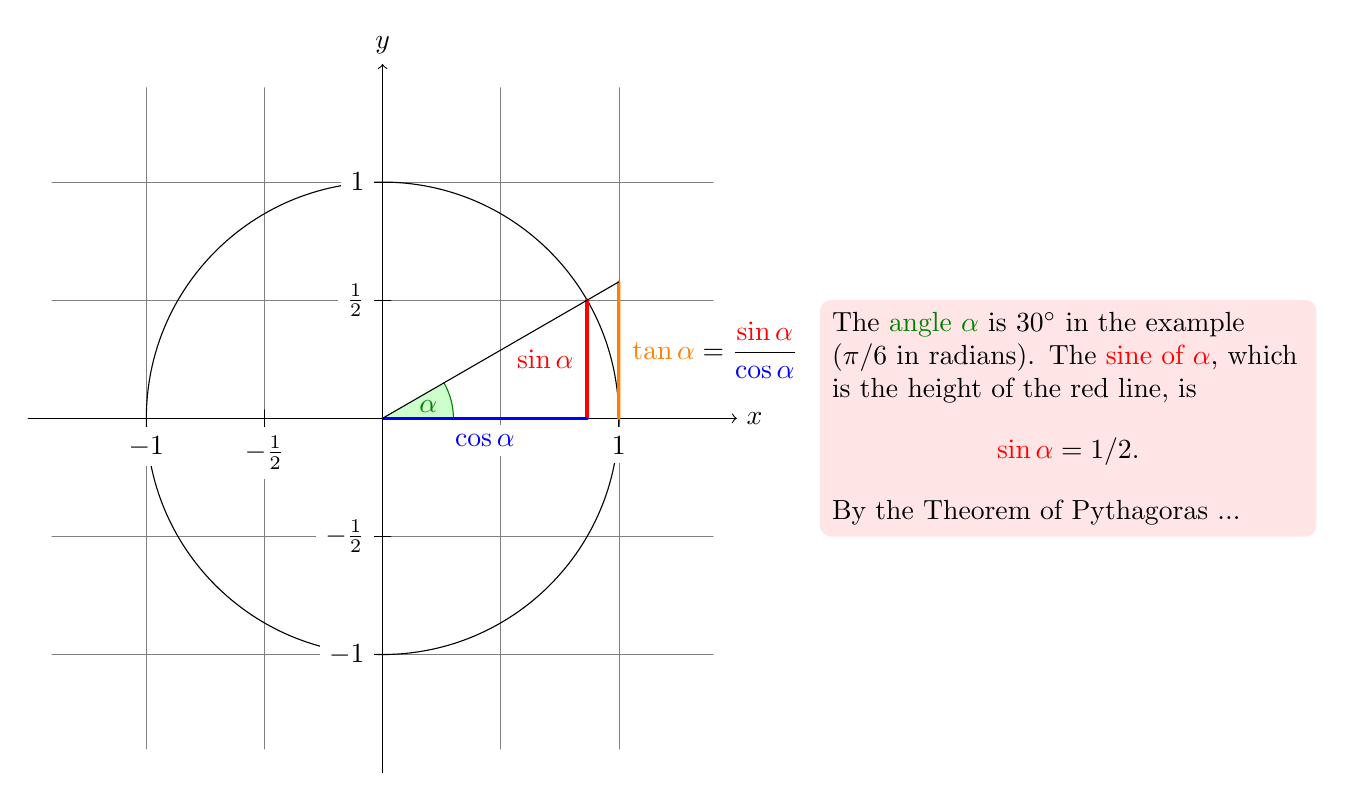
\begin{tikzpicture}
[scale=3,line cap=round,
% Styles
axes/.style=,
important line/.style={very thick},
information text/.style={rounded corners,fill=red!10,inner sep=1ex}]
% Local definitions
\def\costhirty{0.8660256}
% Colors
\colorlet{anglecolor}{green!50!black}
\colorlet{sincolor}{red}
\colorlet{tancolor}{orange!80!black}
\colorlet{coscolor}{blue}
% The graphic
\draw[help lines,step=0.5cm] (-1.4,-1.4) grid (1.4,1.4);
\draw (0,0) circle (1cm);
\begin{scope}[axes]
\draw[->] (-1.5,0) -- (1.5,0) node[right] {$x$} coordinate(x axis);
\draw[->] (0,-1.5) -- (0,1.5) node[above] {$y$} coordinate(y axis);
\foreach \x/\xtext in {-1, -.5/-\frac{1}{2}, 1}
\draw[xshift=\x cm] (0pt,1pt) -- (0pt,-1pt) node[below,fill=white] {$\xtext$};
\foreach \y/\ytext in {-1, -.5/-\frac{1}{2}, .5/\frac{1}{2}, 1}
\draw[yshift=\y cm] (1pt,0pt) -- (-1pt,0pt) node[left,fill=white] {$\ytext$};
\end{scope}
\filldraw[fill=green!20,draw=anglecolor] (0,0) -- (3mm,0pt) arc(0:30:3mm);
\draw (15:2mm) node[anglecolor] {$\alpha$};
\draw[important line,sincolor]
(30:1cm) -- node[left=1pt,fill=white] {$\sin \alpha$} (30:1cm |- x axis);
\draw[important line,coscolor]
(30:1cm |- x axis) -- node[below=2pt,fill=white] {$\cos \alpha$} (0,0);
\path [name path=upward line] (1,0) -- (1,1);
\path [name path=sloped line] (0,0) -- (30:1.5cm);
\draw [name intersections={of=upward line and sloped line, by=t}]
[very thick,orange] (1,0) -- node [right=1pt,fill=white]
{$\displaystyle \tan \alpha \color{black}=
\frac{{\color{red}\sin \alpha}}{\color{blue}\cos \alpha}$} (t);
\draw (0,0) -- (t);
\draw[xshift=1.85cm]
node[right,text width=6cm,information text]
{
The {\color{anglecolor} angle $\alpha$} is $30^\circ$ in the
example ($\pi/6$ in radians). The {\color{sincolor}sine of
$\alpha$}, which is the height of the red line, is
\[
{\color{sincolor} \sin \alpha} = 1/2.
\]
By the Theorem of Pythagoras ...
};
\end{tikzpicture}

Top align:
\tikz[baseline=1.5ex]
\draw (0,0) rectangle (1cm,4ex);

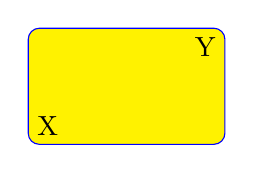
\begin{tikzpicture}[execute at end picture=%
  {
    \begin{pgfonlayer}{background}
      \path[draw=blue,fill=yellow,rounded corners]
      (current bounding box.south west) rectangle
      (current bounding box.north east);
    \end{pgfonlayer}
  }]
  \node at (0,0) {X};
  \node at (2,1) {Y};
\end{tikzpicture}

\end{document}
